\section{Approach}
\label{sec:approach}
In this section, we first describe our methodology for 
cause-effect pairs extraction. 
Then we demonstrate the causal attention as well as its fusion mechanism with the soft attention based on the CNN seq2seq model for commonsense causality generation.

\subsection{Cause-Effect Pairs Extraction}
\label{sec:causal_pairs}
The sentences are the basic semantic units which completely describe the events with both \emph{agents} and \emph{actions}.
Therefore, to study the causal sentence generation task, we build a new dataset of cause-effect sentence pairs from novels~\footnote{We describe this corpus in detail in \secref{sec:eval}.} by extracting main and subordinate clauses connected by causal conjunctions (i.e., ``because'' and ``so''). 
We perform the extraction as follows:

\begin{figure}[t!]
	\centering
	\includegraphics[width=\columnwidth]{parse.pdf}
	\caption{Cause and effect sentence extracted from a sample sentence after coreference resolution, along with its constituent parse tree. Nodes coloured in light orange are those critical for syntactical checking in our extraction process.}
	\label{fig:parse}
\end{figure}
\begin{itemize}
	\item Cue Sentences Collection. 
	We first collect sentences containing ``because'' or ``so'' by regular expression matching. Those sentences are fed into Stanford CoreNLP~\cite{stanfordcorenlp} tools for tokenization, POS tagging, constituent parsing and dependency parsing.
	\item Negation Detection. 
	If the causal conjunction node in dependency tree
	has a negation word sibling such as ``not'' and ``n't'', 
	we do not consider this sentence for further extraction.
	\item Clause Detection. 
	We design syntactic pattern matching rules for 
	cause-effect sentence pairs extraction.
	 Basically we make sure the "because" in the sentence is a subordinate conjunction word leading a subordinate clause(tagged as `SBAR'), which contains a declarative 
	sentence(`S') with subject(`NP') and predicate(`VP').
	Similarly, we design the syntactic rules for the `so that' pattern.
	We further demonstrate such syntactic rules in \figref{fig:parse}.
	
	\item Spans Extraction. 
	We remove redundant punctuations and unwanted sentence
	constituents from the subtree of the main clause and that of the subordinate clause. Then, the text spans contained by those subtrees are extracted as cause-effect sentence pairs.
%	\item (Partial) Coreference Resolution. The order of cause/effect span is determined by the causal conjunction. Take ``because'' as an example, the order is always ``EFFECT because CAUSE'', resulting in representative mention in effect sentence but 
%	pronouns in cause. Therefore, we substitute pronouns in subordinate clause with the representative mention in main clause for each causal pair to enable bidirectional 
%	inference. We don't do coreference resolution on the whole sentence to avoid unnecessary repetition. 

\end{itemize}

\textbf{Input Transformations.} 
We create two data examples from each cause-effect sentence pair for both forward causal reasoning and backward causal reasoning.
While training, we add the special token $\left< f\right>$ or $\left< b \right>$ in front of the target span to indicate the forward or backward reasoning example.
When testing, we initialize the first token of the generated sequence as $\left< f\right>$ or $\left< b \right>$  to perform the forward reasoning or backward reasoning separately.

Note that, we also do the co-reference resolution for the cue sentences, since we create both forward and backward reasoning examples. 
%Finally, we create two source/target pairs from the example sentence shown in \figref{fig:parse} (\tabref{tab:example}).
Finally, as shown in \figref{fig:example}, we create two source/target pairs 
from the example sentenc of \figref{fig:parse}.
\cut{%%%%%%%%
\textbf{Forward:}
 \begin{itemize}
	\item [] source sequence: Amanda feels hot
	\item [] target sequence: $\left< f\right>$ Amanda turns on the fan
\end{itemize}

\textbf{Backward:}
\begin{itemize}
	\item [] source sequence: Amanda turns on the fan
	\item [] target sequence: $\left< b\right>$ Amanda feels hot
\end{itemize}
%\YZ{co-reference}
\begin{table*}[th]
    \centering
    \begin{tabular}{|c|l|l|}%{|p{7cm}|rl|}
    \hline
         & Forward & Backward \\ \hline
    Source & Amanda feels hot & Amanda turns on the fan \\ \hline
    Target & $\left< f\right>$ Amanda turns on the fan &  $\left< b\right>$ Amanda feels hot \\ \hline
    \end{tabular}
    \caption{The cause-effect sentence pair for forward and backward causal reasoning.}
    \label{tab:example}
\end{table*}
}%%%%%%%%%%%%%%
\begin{figure*}[th!]
\centering
\subfigure[Forward]{
\includegraphics[width=0.8\linewidth]{for}
}
\quad
\subfigure[Backward]{
\includegraphics[width=0.8\linewidth]{back}
}
\caption{The cause-effect pair for forward and backward causal reasoning.}
\label{fig:example}
\end{figure*}


\subsection{Background: CNN Seq2seq Model}
\label{sec:cnn}
In this section, we briefly introduce the convolutional sequence to sequence (CNN seq2seq\footnote{\url{https://github.com/facebookresearch/fairseq-py}}) model which applies on causality generation as a baseline model and later we implement our proposed attention mechanism on this model.

%\begin{figure}[th]
%	\centering
%	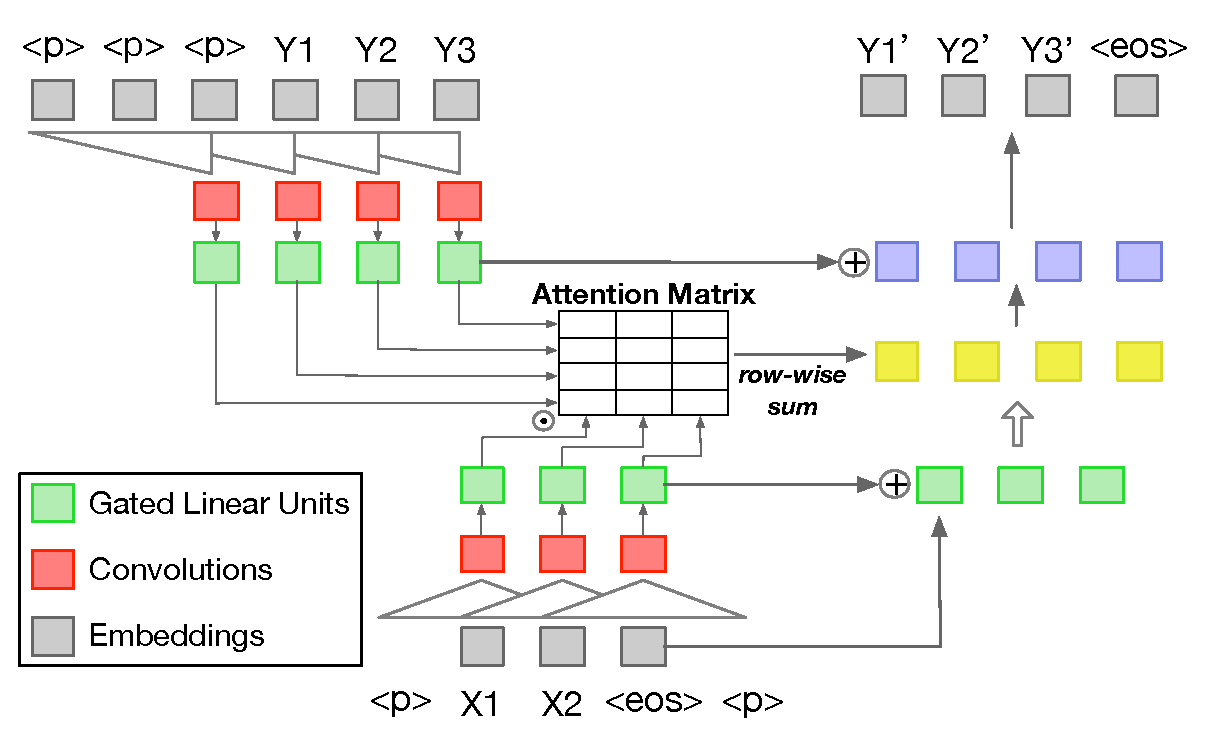
\includegraphics[width=1.0\columnwidth]{cnn}
%	\caption{Convolutional seq2seq model. }
%	\label{fig:basicModel}
%\end{figure}
%
%The CNN seq2seq model includes multi-layer convolutional seq2seq networks \cite{gehring2017convs2s} and attention mechanism \footnote{\url{https://github.com/facebookresearch/fairseq-py}}
%(\figref{fig:basicModel}).

In CNN seq2seq models, given the input elements $\textbf{x} = (x_{1},x_{2},...,x_{m})$ and 
output elements $\textbf{y} = (y_{1}, y_{2},..., y_{n})$ ($m>n$),
we obtain the input representations  $\mathbf{X} = (X_1,...,X_m)$ 
and output representations $\mathbf{Y}=(Y_1,...,Y_n)$ by combining
word embeddings and their corresponding position embeddings vectors. 
$\mathbf { z } ^ { l } = \left( z _ { 1 } ^ { l } , \ldots , z _ { m } ^ { l } \right)$ and $\mathbf { h } ^ { l } = \left( h _ { 1 } ^ { l } , \ldots , h _ { n } ^ { l } \right)$ 
are convolutional output of the encoder and decoder in the $l$-th layer.
We use GLU \cite{DauphinFAG17} and residual connections \cite{HeZRS16} after convolution 
in each layer to ensure that the sufficient and effective information is transmitted layer by layer.  
\begin{equation}
%\small
h _ { i } ^ { l } = ~ GLU \left( W ^ { l } \left[ h _ {i-k/2 } ^ { l - 1 } , \ldots , h _ { i+k/2 } ^ { l - 1 } \right] + b _ { w } ^ { l } \right)  + h _ { i } ^ { l - 1 }
\end{equation} 
where \textit{k} is kernel width.
We compute the probability
distribution of generating the next elements $y_{i+1}$
based on the current state and transform the top
decoder output $h_{i}^{l}$ via softmax:
%\begin{equation}
%%\small
%\begin{split}
%p \left( y _ { i + 1 } | y _ { 1 } , \ldots , y _ { i } , \mathbf { x } \right) = 
%& \operatorname { softmax } \left( W _ { o } h _ { i } ^ { L } + b _ { o } \right) \\ 
%&\in \mathbb { R } ^ { T }
%\end{split}
%\end{equation}
\begin{equation}
%\small
p \left( y _ { i + 1 } | y _ { 1 } , \ldots , y _ { i } , \mathbf { x } \right) = 
 \operatorname { softmax } \left( W _ { o } h _ { i } ^ { L } + b _ { o } \right) \\ 
\in \mathbb { R } ^ { T }
\end{equation}
For each decoder layer, 
we combine the current decoder state $h_{i}$
with an embedding of the previous target element via $Y_{i}$:
\begin{equation}
%\small
d _ { i } ^ { l } = W _ { d } ^ { l } h _ { i } ^ { l } + b _ { d } ^ { l } + Y _ { i }
\end{equation}

The conditional input to the current 
decoder layer is a weighted sum of both encoder states and input element representations.
\begin{equation}\label{eq:a}
%\small
a _ { i j } ^ { l } = \frac { \exp \left( d _ { i } ^ { l } \cdot z _ { j } ^ { u } \right) } { \sum _ { t = 1 } ^ { m } \exp \left( d _ { i } ^ { l } \cdot z _ { t } ^ { u } \right) }
\end{equation}
\begin{equation}\label{eq:c}
%\small
c _ { i } ^ { l } = \sum _ { j = 1 } ^ { m } a _ { i j } ^ { l } \left( z _ { j } ^ { u } + X_j \right)
\end{equation}
%where $z_{j}^{u}$ is the encoder output of last layer $u$.  
where $u$ is the last layer of encoder.  
Finally, $c _ { i } ^ { l }$ is added to $h_{i}^{l}$ as the input for the next decoder layer.


\subsection{Causal Attention}
\label{sec:causal_attention}
The CNN seq2seq model for causality generation is trained
on the extracted cause-effect pairs described in \secref{sec:causal_pairs}. 
Such pairs are extracted by the `because` and `so that` cue patterns. 
The scarcity and the noise of the training pairs raises the
question of whether the CNN seq2seq model can learn a strong enough causal dependency model for causality generation.
To ameliorate this limitation, we propose a causal attention 
mechanism which leverages external causal knowledge, CausalNet~\cite{LuoSZHW16}, to complement the global causal dependency guidance for causality generation.

Luo et al.~\cite{LuoSZHW16} harvest the causal evidences from web-scale corpus, and backed by this network, the causal strength metric is proposed to measure the causal
strength between short texts including words, phrases and sentences. 
Thus, the causal strength from CausalNet reflects the commonsense causal dependency between short texts.
We model the causal dependency as an alignment
mechanism (i.e. attention mechanism) in the sequence to sequence framework.
Specifically, we use the word-level causal strengths (i.e. $cs$)~\cite{LuoSZHW16} in logarithm space as the causal attention scores.
The logarithm causal strength (i.e. $CS$) between $y_i$ and $x_j$ is computed as:
%\begin{equation}\label{eq:acs}
%	\begin{split}
%	CS(y_i, x_j)  & =  \log\left(cs(y_i,x_j)\right) \\
%		& - \log\left(min\{cs(\cdot, \cdot)\}\right)
%	\end{split}
%\end{equation}
\begin{equation}\label{eq:acs}
CS(y_i, x_j) = \log\left(cs(y_i,x_j)\right) - \log\left(min\{cs(\cdot, \cdot)\}\right)
\end{equation}
%\begin{equation}
%\label{eq:causal_attn}
%a^{l} _ { i j }= Softmax\left( CS(y_i, x_j) \right) ,
%\end{equation}
where $y_i$ is $i$-th word in encoder input, 
and $x_j$ is $j$-th word in decoder output.

For the vanilla causal attention mechanism, 
we attempt to replace the attention scores $a^l_{ij}$ in \eqnref{eq:a} with $Softmax\left( CS(y_i, x_j) \right)$.
So far, there is one problem for such directly substitution.
The conventional soft attention scores at the $i$-th decoding time step  (i.e. $a^{l}_{ij}$) is computed from the hidden states $d^l_i$ and $z^l_j$. 
Unlike the conventional soft attention,
the causal attention scores are not computed from the hidden states.
To retrieve the causal strengths at the $i$-th decoding time step, we need to know both the source word (i.e. $x_j$) as well as the target word (i.e. $y_i$) in advance.
It is easy to obtain the causal attention scores while training since we know the golden targets.
However, we do not know the target word in advance
at the inferencing time. 

We solve this problem by introducing the
trainable parameters $\mathbf{w_p}$ to average causal strengths $CS(y_{\cdot}, x_j)$ over all the words in target vocabulary $V^t$. We use $\mathbf{cs}(x_j)$ to represent
the causal strength vector, where  the $i$-th element of $\mathbf{cs}(x_j)$ is $CS(V^t_i, x_j)$.
Then, we compute the causal attention scores $ca^l_{ij}$ as following:
\begin{equation}
\label{eq:ca} % causal attention scores
ca^{l} _ { i j }= Softmax\left( \mathbf{w_p} \cdot
\mathbf{cs}(x_j) \right) ,
\end{equation}
We substitute $ca^{l} _ { i j }$ in~\eqnref{eq:ca} for the $a^l_{ij}$ in~\eqnref{eq:a}.
This forms the causal attention baseline model denoted as
$CS_{only}$ in our experiments.

%We compute the context vector in \eqref{eq:c} as following:
%\begin{equation}
%%\begin{split}
%\mathbf{c_i} = p^{(i)}_{cs}\mathbf{w_{cs}}\sum_{j=1}^{m}\mathbf{v_{\boldsymbol{\cdot} j}} \times \mathbf{z_j}  + (1-p^{(i)}_{cs})\mathbf{e_i}
%%\end{split}
%\end{equation}
%\begin{equation}
%\mathbf{e_i} = \sum_{j=1}^{m}a_{ij}\mathbf{z_j},
%\end{equation}
%where $\mathbf{e_i}$ is the context vector when decoding at the $i$-th time step. 
%$v_{\cdot j}$ is the causal strength vector with $V \times 1$ dimension  $\mathbf{w_{cs}}$ is 



%\subsection{Causality Fused Attention Mechanism}
\subsection{Attention Fusion Mechanism}
\label{sec:fusion}
In the previous section, causal attention
carries the causal dependency globally harvested from CausalNet~\cite{LuoSZHW16}.
However, such global causal dependency does not change across different layers which loses the hierarchical semantic attending information.
The soft attention in CNN seq2seq model learns the 
local causal dependency while training.
Thus, we propose an attention fusion mechanism 
to fuse the causal attention with the stacked soft attention, equipping the sequence to sequence model with global causal information.
In this section, we describe the attention fusion mechanism used for our experiments.

%To facilitate causality generation, we propose \emph{causal weighing} $P_{cs}$ to fuse the global causal attention 
%with soft attention, changing \eqnref{eq:a} and \eqnref{eq:c} as follows:

The soft attention and causal attention proposed in ~\secref{sec:causal_attention} separately encodes the local and global causal dependency between the source text and the target text.
To make the model more expressive, 
we combine the global causal dependency with the local causal dependency using a weighting scheme.
We implement this by weighing the causal attention scores
$ca^l_{ij}$ and the soft attention scores $sa^l_{ij}$ through  $\lambda_{cs}$ called \emph{causal fusion weight}.
The fused attention score $fa^l_{ij}$ is computed as follows:
\begin{equation}
\label{eq:fusion}
fa^l_{ij} = \lambda_{cs} \cdot ca^l_{ij} + (1-\lambda_{cs}) \cdot sa^l_{ij}
\end{equation}
$\lambda_{cs}$ represents the weight of causal attention score, controlling the influence of global causal information in the model.
$ca^l_{ij}$ and $sa^l_{ij}$ are calculated as shown in
~\eqnref{eq:ca} and ~\eqnref{eq:a} separately.
We compute $\lambda^l_{cs}$ as follows:
\begin{equation}
\label{eq:weight}
\lambda^l_{cs} = \sigma(w^l),
\end{equation}
where $\sigma$ denotes the sigmoid function which 
normalizes $\lambda^l_{cs}$ between 0 and 1
and $w^l$ denotes the learnable parameter in the model.
We design the causal fusion weight $\lambda^l_{cs}$ as the normalized trainable parameter
to make the weighing scheme more flexible.  
Our causal attention fusion mechanism aggregates causal information from the global and local causal dependency to refine the decoding at every time step. 
We illustrate the proposed attention fusion mechanism
as shown in~\figref{fig:fusedatt}.

\subsection{Fine-tuning Procedure}
We can perform our model on the datasets across sources and domains by a straightforward fine-tuning procedure.

As we described, we train the commonsense causality
generation model on the extracted cause-effect pairs
from novels (see details in \secref{sec:xx}). 
We initialize the parameters with this pre-trained model and effectively perform fine-tuning with a minimal data examples from other sources or domains. 
We show the effectiveness of our fine-tuned model in
~\secref{sec:xx}.

%\begin{equation}
%\begin{split}
%c_i = & ~P^{(i)}_{cs}W_{cs}\sum_{j=1}^{m}CS(y_i,x_j)z_{ij} \\
%		& + (1-P^{(i)}_{cs})e_i 
%\end{split}
%\end{equation}

%\begin{equation}
%\mathbf{c_i} = p^{(i)}_{cs}\mathbf{w_{cs}}\sum_{j=1}^{m}\mathbf{v_{\boldsymbol{\cdot} j}} \times \mathbf{z_j}  + (1-p^{(i)}_{cs})\mathbf{e_i}

%\end{equation}
%\begin{equation}
%\mathbf{e_i} = \sum_{j=1}^{m}a_{ij}\mathbf{z_j},
%\end{equation}
%where $\mathbf{e_i}$ is the context vector when decoding at the $i$-th time step. 
%$v_{\cdot j}$ is the causal strength vector with $V \times 1$ dimension  $\mathbf{w_{cs}}$ is 

\begin{figure*}[th]
    \centering
    \includegraphics[width=2\columnwidth]{fusedatt2}
    \caption{Causality Fused attention. }
    \label{fig:fusedatt}
\end{figure*}

%The causality fused attention mechanism is illustrated in \figref{fig:fusedatt}.
%Compared with Global and Easy Combination methods, the advatages
%of Fusion attention is that this model has the ability to 
%obtain the causality information and generate correct text according
%to desired \textit{marks} in its inner state.

